\documentclass{article}
\usepackage[utf8]{inputenc}
\usepackage{geometry}
\usepackage{graphicx}
\usepackage{amsmath}
\usepackage{amsfonts}
\usepackage{amsthm}
\usepackage{amssymb}
\usepackage[most]{tcolorbox}
\usepackage{array}
\usepackage{latexsym}
\usepackage{alltt}
\usepackage{hyperref}
\usepackage{color}
\usepackage{float}
\usepackage{pdfpages}
\usepackage{algpseudocode}
\usepackage{multicol}
\usepackage{multirow}
\usepackage{caption}
\usepackage{xparse}
\usepackage{setspace}
\usepackage{enumitem}
\usepackage{tikz}
\usepackage{pdflscape}


\geometry
{
  a4paper,
  left=5mm,
  right=5mm,
  top=5mm,
  bottom=5mm,
}

% mybox
\newtcolorbox{mybox}[3][]
{
  colframe = #2!25,
  colback  = #2!10,
  coltitle = #2!20!black,  
  title    = {#3},
  #1,
}

% New environments that use mybox
\newenvironment{example}[1]{\begin{mybox}{green}{\textbf{Example #1}}}{\end{mybox}}
\newenvironment{example_break}[1]{\begin{mybox}[breakable]{green}{\textbf{Example #1}}}{\end{mybox}}
\newenvironment{definition}[1]{\begin{mybox}{blue}{\textbf{Definition #1}}}{\end{mybox}}
\newenvironment{theorem}[1]{\begin{mybox}{red}{\textbf{Theorem #1}}}{\end{mybox}}
\newenvironment{formula}[1]{\begin{mybox}{red}{\textbf{#1}}}{\end{mybox}}

% Changing maketitle
\makeatletter         
\renewcommand\maketitle{
{\raggedright % Note the extra {
\begin{center}
{\Large \bfseries \@title}\\[2ex] 
{\large \@author \ - \@date}\\[2ex]
\end{center}}} % Note the extra }
\makeatother

% \onehalfspacing % adjust spacing

% macros
\newcommand{\prob}[1]{\textbf{\textit{P}}\{#1\}}
\NewDocumentCommand{\dsum}{%
    e{^_}
}{%
  {% 
    \displaystyle\sum
    \IfValueT{#1}{^{#1}}
    \IfValueT{#2}{_{#2}}
  }
}%

% maketitle variables
\title{Title}
\author{Burak Metehan Tunçel}
\date{\today}

\begin{document}

\section*{Student Information}

Name : Burak Metehan Tunçel\\
ID : 2468726\\

\section*{Answer 1}

\subsection*{a)}

The regular expression:
\begin{equation*}
  \left( \left( a \cup b \right)^* aa \left(a \cup b \right)^* bb \left( a \cup b \right)^* \right) \cup \left( \left( a \cup b \right)^* bb \left(a \cup b \right)^* aa \left( a \cup b \right)^* \right)
\end{equation*}
This is equivalent to:
\begin{equation*}
  (a \cup b)^* ((aa (a \cup b)^* bb) \cup (bb (a \cup b)^* aa)) (a \cup b)^*
\end{equation*}

\subsection*{b)}

Formally define and draw an NFA that recognizes the language.

Let M be a NFA:
\begin{equation*}
  M = (K, \Sigma, \Delta, s, F)
\end{equation*}
where,
\begin{itemize}
  \item $K = \{ q_{0}, q_{1}, q_{2}, q_{3}, q_{4}, q_{5}, q_{6}, q_{7}, q_{8}, q_{9}, q_{10}, q_{11} \}$
  \item $\Sigma = \{ a, b \}$
  \item $s = q_0$, the initial state
  \item $F = \{ q_{11} \}$, final states
  \item The transition relation$\Delta = \left\{ \begin{aligned}
      &(q_0, a, q_1), (q_0, b, q_1), (q_0, e, q_1), (q_1, e, q_0), (q_1, a, q_2), (q_1, b, q_6),\\
      &(q_2, a, q_3), (q_3, a, q_4), (q_3, b, q_4), (q_3, e, q_4), (q_4, e, q_3), (q_4, b, q_5),\\
      &(q_5, b, q_{10}), (q_6, b, q_7), (q_7, a, q_8), (q_7, b, q_8), (q_7, e, q_8), (q_8, e, q_7),\\
      &(q_8, a, q_9), (q_9, a, q_{10}), (q_{10}, a, q_{11}), (q_{10}, b, q_{11}), (q_{10}, e, q_{11}), (q_{11}, e, q_{10}) \}
    \end{aligned} \right\}$
\end{itemize}

The NFA $M$:
\begin{figure}[ht!]
  \centering
  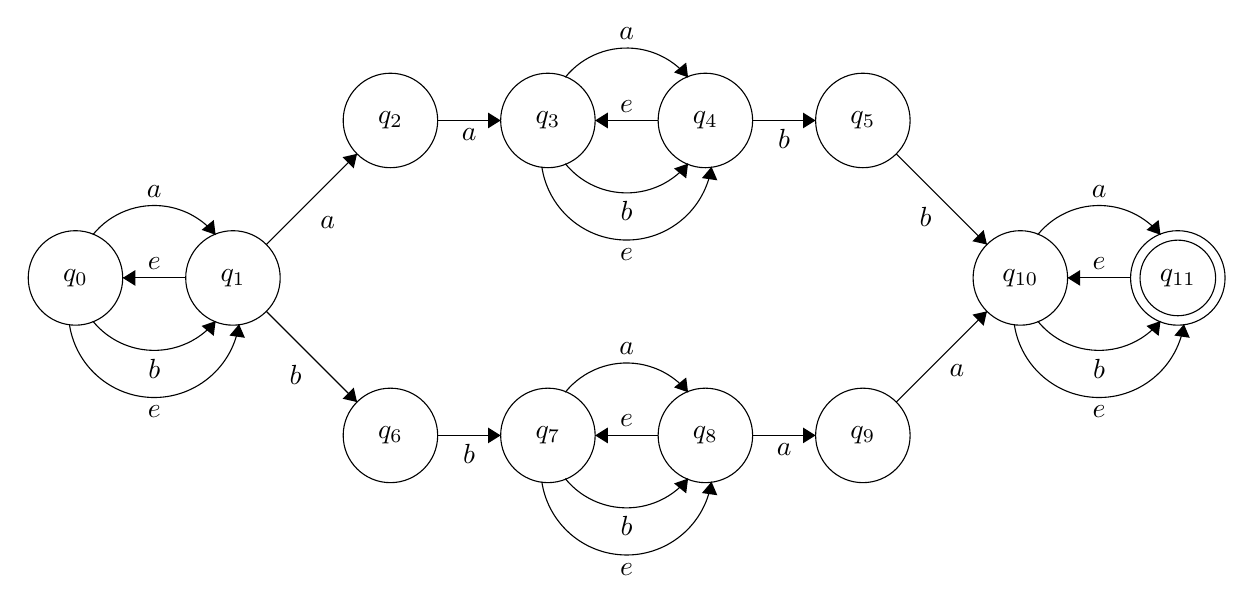
\begin{tikzpicture}[scale=0.2]
    \tikzstyle{every node}+=[inner sep=0pt]
    \draw [black] (3.3,-16.5) circle (3);
    \draw (3.3,-16.5) node {$q_0$};
    \draw [black] (13.3,-16.5) circle (3);
    \draw (13.3,-16.5) node {$q_1$};
    \draw [black] (23.3,-6.5) circle (3);
    \draw (23.3,-6.5) node {$q_2$};
    \draw [black] (33.3,-6.5) circle (3);
    \draw (33.3,-6.5) node {$q_3$};
    \draw [black] (43.3,-6.5) circle (3);
    \draw (43.3,-6.5) node {$q_4$};
    \draw [black] (53.3,-6.5) circle (3);
    \draw (53.3,-6.5) node {$q_5$};
    \draw [black] (23.3,-26.5) circle (3);
    \draw (23.3,-26.5) node {$q_6$};
    \draw [black] (33.3,-26.5) circle (3);
    \draw (33.3,-26.5) node {$q_7$};
    \draw [black] (43.3,-26.5) circle (3);
    \draw (43.3,-26.5) node {$q_8$};
    \draw [black] (53.3,-26.5) circle (3);
    \draw (53.3,-26.5) node {$q_9$};
    \draw [black] (63.3,-16.5) circle (3);
    \draw (63.3,-16.5) node {$q_{10}$};
    \draw [black] (73.3,-16.5) circle (3);
    \draw (73.3,-16.5) node {$q_{11}$};
    \draw [black] (73.3,-16.5) circle (2.4);
    \draw [black] (4.402,-13.758) arc (140.97764:39.02236:5.017);
    \fill [black] (12.2,-13.76) -- (12.08,-12.82) -- (11.31,-13.45);
    \draw (8.3,-11.4) node [above] {$a$};
    \draw [black] (12.198,-19.242) arc (-39.02236:-140.97764:5.017);
    \fill [black] (12.2,-19.24) -- (11.31,-19.55) -- (12.08,-20.18);
    \draw (8.3,-21.6) node [below] {$b$};
    \draw [black] (13.685,-19.437) arc (-8.31382:-171.68618:5.443);
    \fill [black] (13.69,-19.44) -- (13.08,-20.16) -- (14.06,-20.3);
    \draw (8.3,-24.59) node [below] {$e$};
    \draw [black] (15.42,-14.38) -- (21.18,-8.62);
    \fill [black] (21.18,-8.62) -- (20.26,-8.83) -- (20.97,-9.54);
    \draw (18.82,-12.98) node [right] {$a$};
    \draw [black] (10.3,-16.5) -- (6.3,-16.5);
    \fill [black] (6.3,-16.5) -- (7.1,-17) -- (7.1,-16);
    \draw (8.3,-16) node [above] {$e$};
    \draw [black] (26.3,-6.5) -- (30.3,-6.5);
    \fill [black] (30.3,-6.5) -- (29.5,-6) -- (29.5,-7);
    \draw (28.3,-7) node [below] {$a$};
    \draw [black] (34.402,-3.758) arc (140.97764:39.02236:5.017);
    \fill [black] (42.2,-3.76) -- (42.08,-2.82) -- (41.31,-3.45);
    \draw (38.3,-1.4) node [above] {$a$};
    \draw [black] (42.198,-9.242) arc (-39.02236:-140.97764:5.017);
    \fill [black] (42.2,-9.24) -- (41.31,-9.55) -- (42.08,-10.18);
    \draw (38.3,-11.6) node [below] {$b$};
    \draw [black] (43.685,-9.437) arc (-8.31382:-171.68618:5.443);
    \fill [black] (43.69,-9.44) -- (43.08,-10.16) -- (44.06,-10.3);
    \draw (38.3,-14.59) node [below] {$e$};
    \draw [black] (40.3,-6.5) -- (36.3,-6.5);
    \fill [black] (36.3,-6.5) -- (37.1,-7) -- (37.1,-6);
    \draw (38.3,-6) node [above] {$e$};
    \draw [black] (46.3,-6.5) -- (50.3,-6.5);
    \fill [black] (50.3,-6.5) -- (49.5,-6) -- (49.5,-7);
    \draw (48.3,-7) node [below] {$b$};
    \draw [black] (55.42,-8.62) -- (61.18,-14.38);
    \fill [black] (61.18,-14.38) -- (60.97,-13.46) -- (60.26,-14.17);
    \draw (57.28,-11.98) node [below] {$b$};
    \draw [black] (64.402,-13.758) arc (140.97764:39.02236:5.017);
    \fill [black] (72.2,-13.76) -- (72.08,-12.82) -- (71.31,-13.45);
    \draw (68.3,-11.4) node [above] {$a$};
    \draw [black] (72.198,-19.242) arc (-39.02236:-140.97764:5.017);
    \fill [black] (72.2,-19.24) -- (71.31,-19.55) -- (72.08,-20.18);
    \draw (68.3,-21.6) node [below] {$b$};
    \draw [black] (73.685,-19.437) arc (-8.31382:-171.68618:5.443);
    \fill [black] (73.69,-19.44) -- (73.08,-20.16) -- (74.06,-20.3);
    \draw (68.3,-24.59) node [below] {$e$};
    \draw [black] (70.3,-16.5) -- (66.3,-16.5);
    \fill [black] (66.3,-16.5) -- (67.1,-17) -- (67.1,-16);
    \draw (68.3,-16) node [above] {$e$};
    \draw [black] (15.42,-18.62) -- (21.18,-24.38);
    \fill [black] (21.18,-24.38) -- (20.97,-23.46) -- (20.26,-24.17);
    \draw (17.28,-21.98) node [below] {$b$};
    \draw [black] (26.3,-26.5) -- (30.3,-26.5);
    \fill [black] (30.3,-26.5) -- (29.5,-26) -- (29.5,-27);
    \draw (28.3,-27) node [below] {$b$};
    \draw [black] (34.402,-23.758) arc (140.97764:39.02236:5.017);
    \fill [black] (42.2,-23.76) -- (42.08,-22.82) -- (41.31,-23.45);
    \draw (38.3,-21.4) node [above] {$a$};
    \draw [black] (42.198,-29.242) arc (-39.02236:-140.97764:5.017);
    \fill [black] (42.2,-29.24) -- (41.31,-29.55) -- (42.08,-30.18);
    \draw (38.3,-31.6) node [below] {$b$};
    \draw [black] (43.685,-29.437) arc (-8.31382:-171.68618:5.443);
    \fill [black] (43.69,-29.44) -- (43.08,-30.16) -- (44.06,-30.3);
    \draw (38.3,-34.59) node [below] {$e$};
    \draw [black] (40.3,-26.5) -- (36.3,-26.5);
    \fill [black] (36.3,-26.5) -- (37.1,-27) -- (37.1,-26);
    \draw (38.3,-26) node [above] {$e$};
    \draw [black] (46.3,-26.5) -- (50.3,-26.5);
    \fill [black] (50.3,-26.5) -- (49.5,-26) -- (49.5,-27);
    \draw (48.3,-27) node [below] {$a$};
    \draw [black] (55.42,-24.38) -- (61.18,-18.62);
    \fill [black] (61.18,-18.62) -- (60.26,-18.83) -- (60.97,-19.54);
    \draw (59.27,-21.98) node [below] {$a$};
  \end{tikzpicture}
  \caption{$M$}  
\end{figure}


\newpage
\subsection*{c)}

We want to construct DFA. In other words we want to acquire:
\begin{equation*}
    M' = (K', \Sigma, \delta', s', F')
\end{equation*}

While constructing a DFA from an NFA, $E(q)$ should be computed for $q \in K$. Instead of doing this, I will compute $E(q)$ for some, or all, $q \in K$ when it is needed. Also, it can be decided that $s' = q_{100}$

We start from the initial state of DFA, $s' = q_{100} = E(q_0)$.

\begin{equation*}
    E(q_{0}) = \{ q_{0}, q_{1} \}
\end{equation*}

\begin{equation*}
    (q_{0}, a, q_{1}), (q_{1}, a, q_{2})
\end{equation*}

\noindent are all the transitions $(q, a, p)$ for some $q \in E(q_{0})$. It follows that

\begin{equation*}
    \delta'(q_{100}, a) = E(q_{1}) \cup E(q_{2})
\end{equation*}

\noindent I need to compute $E(q_{1}), E(q_{2})$:
\begin{itemize}
    \item $E(q_{1}) = \{ q_{0}, q_{1} \}$
    \item $E(q_{2}) = \{ q_{2} \}$
\end{itemize}

\begin{align*}
    \delta'(q_{100}, a) = \{ q_{0}, q_{1}, q_{2} \}
\end{align*}

\noindent There is a new state. Let the state be $q_{101}$. Similarly,

\begin{equation*}
    (q_{0}, b, q_{1}), (q_{1}, b, q_{6})
\end{equation*}

\noindent are all the transitions $(q, b, p)$ for some $q \in E(q_{0})$. It follows that

\begin{equation*}
    \delta'(q_{100}, b) = E(q_{1}) \cup E(q_{6})
\end{equation*}

\noindent I have $E(q_{1})$. I need to compute $E(q_{6})$:
\begin{itemize}
    \item $E(q_{6}) = \{ q_{6} \}$
\end{itemize}

\begin{align*}
    \delta'(q_{100}, b) = \{ q_{0}, q_{1}, q_{6} \}
\end{align*}

\noindent There is a new state. Let the state be $q_{102}$.

\begin{formula}{New States and Transitions}
    \textbf{States:}
        \begin{itemize}
            \item $q_{101} = \{ q_{0}, q_{1}, q_{2} \}$
            \item $q_{102} = \{ q_{0}, q_{1}, q_{6} \}$
        \end{itemize}
    \textbf{Transitions:}
        \begin{itemize}
            \item $\delta'(q_{100}, a) = q_{101}$
            \item $\delta'(q_{100}, b) = q_{102}$
        \end{itemize}
\end{formula}

\begin{center}
\subsubsection*{$q_{101}$}
\end{center}

Repeating the calculation for newly introduced state $q_{101}$.

\begin{equation*}
    q_{101} = \{ q_{0}, q_{1}, q_{2} \}
\end{equation*}
So,

\begin{equation*}
    E(q_{101}) = \{ q_{0}, q_{1}, q_{2} \}
\end{equation*}

\begin{equation*}
    (q_{0}, a, q_{1}), (q_{1}, a, q_{2}), (q_{2}, a, q_{3})
\end{equation*}

\noindent are all the transitions $(q, a, p)$ for some $q \in E(q_{101})$. It follows that

\begin{equation*}
    \delta'(q_{101}, a) = E(q_{1}) \cup E(q_{2}) \cup E(q_{3})
\end{equation*}

\noindent I have $E(q_{1}), E(q_{2})$. I need to compute $E(q_{3})$:
\begin{itemize}
    \item $E(q_{3}) = \{ q_{3}, q_{4} \}$
\end{itemize}

\begin{align*}
    \delta'(q_{101}, a) = \{ q_{0}, q_{1}, q_{2}, q_{3}, q_{4} \}
\end{align*}

\noindent There is a new state. Let the state be $q_{103}$. Similarly,

\begin{equation*}
    (q_{0}, b, q_{1}), (q_{1}, b, q_{6})
\end{equation*}

\noindent are all the transitions $(q, b, p)$ for some $q \in E(q_{101})$. It follows that

\begin{equation*}
    \delta'(q_{101}, b) = E(q_{1}) \cup E(q_{6})
\end{equation*}

\noindent I have $E(q_{1}), E(q_{6})$. No need to compute anything.

\begin{align*}
    \delta'(q_{101}, b) = \{ q_{0}, q_{1}, q_{6} \}
\end{align*}

\noindent There is not a new state, it is same with the $q_{102}$.

\begin{formula}{New States and Transitions}
    \textbf{States:}
        \begin{itemize}
            \item $q_{103} = \{ q_{0}, q_{1}, q_{2}, q_{3}, q_{4} \}$
        \end{itemize}
    \textbf{Transitions:}
        \begin{itemize}
            \item $\delta'(q_{101}, a) = q_{103}$
            \item $\delta'(q_{101}, b) = q_{102}$
        \end{itemize}
\end{formula}


\begin{center}
\subsubsection*{$q_{102}$}
\end{center}

Repeating the calculation for newly introduced state $q_{102}$.

\begin{equation*}
    q_{102} = \{ q_{0}, q_{1}, q_{6} \}
\end{equation*}
So,

\begin{equation*}
    E(q_{102}) = \{ q_{0}, q_{1}, q_{6} \}
\end{equation*}

\begin{equation*}
    (q_{0}, a, q_{1}), (q_{1}, a, q_{2})
\end{equation*}

\noindent are all the transitions $(q, a, p)$ for some $q \in E(q_{102})$. It follows that

\begin{equation*}
    \delta'(q_{102}, a) = E(q_{1}) \cup E(q_{2})
\end{equation*}

\noindent I have $E(q_{1}), E(q_{2})$. No need to compute anything.

\begin{align*}
    \delta'(q_{102}, a) = \{ q_{0}, q_{1}, q_{2} \}
\end{align*}

\noindent There is not a new state, it is same with the $q_{101}$. Similarly,

\begin{equation*}
    (q_{0}, b, q_{1}), (q_{1}, b, q_{6}), (q_{6}, b, q_{7})
\end{equation*}

\noindent are all the transitions $(q, b, p)$ for some $q \in E(q_{102})$. It follows that

\begin{equation*}
    \delta'(q_{102}, b) = E(q_{1}) \cup E(q_{6}) \cup E(q_{7})
\end{equation*}

\noindent I have $E(q_{1}), E(q_{6})$. I need to compute $E(q_{7})$:
\begin{itemize}
    \item $E(q_{7}) = \{ q_{7}, q_{8} \}$
\end{itemize}

\begin{align*}
    \delta'(q_{102}, b) = \{ q_{0}, q_{1}, q_{6}, q_{7}, q_{8} \}
\end{align*}

\noindent There is a new state. Let the state be $q_{104}$.

\begin{formula}{New States and Transitions}
    \textbf{States:}
        \begin{itemize}
            \item $q_{104} = \{ q_{0}, q_{1}, q_{6}, q_{7}, q_{8} \}$
        \end{itemize}
    \textbf{Transitions:}
        \begin{itemize}
            \item $\delta'(q_{102}, a) = q_{101}$
            \item $\delta'(q_{102}, b) = q_{104}$
        \end{itemize}
\end{formula}


\begin{center}
\subsubsection*{$q_{103}$}
\end{center}

Repeating the calculation for newly introduced state $q_{103}$.

\begin{equation*}
    q_{103} = \{ q_{0}, q_{1}, q_{2}, q_{3}, q_{4} \}
\end{equation*}
So,

\begin{equation*}
    E(q_{103}) = \{ q_{0}, q_{1}, q_{2}, q_{3}, q_{4} \}
\end{equation*}

\begin{equation*}
    (q_{0}, a, q_{1}), (q_{1}, a, q_{2}), (q_{2}, a, q_{3}), (q_{3}, a, q_{4})
\end{equation*}

\noindent are all the transitions $(q, a, p)$ for some $q \in E(q_{103})$. It follows that

\begin{equation*}
    \delta'(q_{103}, a) = E(q_{1}) \cup E(q_{2}) \cup E(q_{3}) \cup E(q_{4})
\end{equation*}

\noindent I have $E(q_{1}), E(q_{2}), E(q_{3})$. I need to compute $E(q_{4})$:
\begin{itemize}
    \item $E(q_{4}) = \{ q_{3}, q_{4} \}$
\end{itemize}

\begin{align*}
    \delta'(q_{103}, a) = \{ q_{0}, q_{1}, q_{2}, q_{3}, q_{4} \}
\end{align*}

\noindent There is not a new state, it is same with the $q_{103}$. Similarly,

\begin{equation*}
    (q_{0}, b, q_{1}), (q_{1}, b, q_{6}), (q_{3}, b, q_{4}), (q_{4}, b, q_{5})
\end{equation*}

\noindent are all the transitions $(q, b, p)$ for some $q \in E(q_{103})$. It follows that

\begin{equation*}
    \delta'(q_{103}, b) = E(q_{1}) \cup E(q_{4}) \cup E(q_{5}) \cup E(q_{6})
\end{equation*}

\noindent I have $E(q_{1}), E(q_{4}), E(q_{6})$. I need to compute $E(q_{5})$:
\begin{itemize}
    \item $E(q_{5}) = \{ q_{5} \} $
\end{itemize}

\begin{align*}
    \delta'(q_{103}, b) = \{ q_{0}, q_{1}, q_{3}, q_{4}, q_{5}, q_{6} \}
\end{align*}

\noindent There is a new state. Let the state be $q_{105}$.

\begin{formula}{New States and Transitions}
    \textbf{States:}
        \begin{itemize}
            \item $q_{105} = \{ q_{0}, q_{1}, q_{3}, q_{4}, q_{5}, q_{6} \}$
        \end{itemize}
    \textbf{Transitions:}
        \begin{itemize}
            \item $\delta'(q_{103}, a) = q_{103}$
            \item $\delta'(q_{103}, b) = q_{105}$
        \end{itemize}
\end{formula}


\begin{center}
\subsubsection*{$q_{104}$}
\end{center}

Repeating the calculation for newly introduced state $q_{104}$.

\begin{equation*}
    q_{104} = \{ q_{0}, q_{1}, q_{6}, q_{7}, q_{8} \}
\end{equation*}
So,

\begin{equation*}
    E(q_{104}) = \{ q_{0}, q_{1}, q_{6}, q_{7}, q_{8} \}
\end{equation*}

\begin{equation*}
    (q_{0}, a, q_{1}), (q_{1}, a, q_{2}), (q_{7}, a, q_{8}), (q_{8}, a, q_{9})
\end{equation*}

\noindent are all the transitions $(q, a, p)$ for some $q \in E(q_{104})$. It follows that

\begin{equation*}
    \delta'(q_{104}, a) = E(q_{1}) \cup E(q_{2}) \cup E(q_{8}) \cup E(q_{9})
\end{equation*}

\noindent I have $E(q_{1}), E(q_{2})$. I need to compute $E(q_{8}), E(q_{9})$:
\begin{itemize}
    \item $E(q_{8}) = \{ q_{7}, q_{8} \}$
    \item $E(q_{9}) = \{ q_{9} \}$
\end{itemize}

\begin{align*}
    \delta'(q_{104}, a) = \{ q_{0}, q_{1}, q_{2}, q_{7}, q_{8}, q_{9} \}
\end{align*}

\noindent There is a new state. Let the state be $q_{106}$. Similarly,

\begin{equation*}
    (q_{0}, b, q_{1}), (q_{1}, b, q_{6}), (q_{6}, b, q_{7}), (q_{7}, b, q_{8})
\end{equation*}

\noindent are all the transitions $(q, b, p)$ for some $q \in E(q_{104})$. It follows that

\begin{equation*}
    \delta'(q_{104}, b) = E(q_{1}) \cup E(q_{6}) \cup E(q_{7}) \cup E(q_{8})
\end{equation*}

\noindent I have $E(q_{1}), E(q_{6}), E(q_{7}), E(q_{8})$. No need to compute anything.

\begin{align*}
    \delta'(q_{104}, b) = \{ q_{0}, q_{1}, q_{6}, q_{7}, q_{8} \}
\end{align*}

\noindent There is not a new state, it is same with the $q_{104}$.

\begin{formula}{New States and Transitions}
    \textbf{States:}
        \begin{itemize}
            \item $q_{106} = \{ q_{0}, q_{1}, q_{2}, q_{7}, q_{8}, q_{9} \}$
        \end{itemize}
    \textbf{Transitions:}
        \begin{itemize}
            \item $\delta'(q_{104}, a) = q_{106}$
            \item $\delta'(q_{104}, b) = q_{104}$
        \end{itemize}
\end{formula}


\begin{center}
\subsubsection*{$q_{105}$}
\end{center}

Repeating the calculation for newly introduced state $q_{105}$.

\begin{equation*}
    q_{105} = \{ q_{0}, q_{1}, q_{3}, q_{4}, q_{5}, q_{6} \}
\end{equation*}
So,

\begin{equation*}
    E(q_{105}) = \{ q_{0}, q_{1}, q_{3}, q_{4}, q_{5}, q_{6} \}
\end{equation*}

\begin{equation*}
    (q_{0}, a, q_{1}), (q_{1}, a, q_{2}), (q_{3}, a, q_{4})
\end{equation*}

\noindent are all the transitions $(q, a, p)$ for some $q \in E(q_{105})$. It follows that

\begin{equation*}
    \delta'(q_{105}, a) = E(q_{1}) \cup E(q_{2}) \cup E(q_{4})
\end{equation*}

\noindent I have $E(q_{1}), E(q_{2}), E(q_{4})$. No need to compute anything.

\begin{align*}
    \delta'(q_{105}, a) = \{ q_{0}, q_{1}, q_{2}, q_{3}, q_{4} \}
\end{align*}

\noindent There is not a new state, it is same with the $q_{103}$. Similarly,

\begin{equation*}
    (q_{0}, b, q_{1}), (q_{1}, b, q_{6}), (q_{3}, b, q_{4}), (q_{4}, b, q_{5}), (q_{5}, b, q_{10}), (q_{6}, b, q_{7})
\end{equation*}

\noindent are all the transitions $(q, b, p)$ for some $q \in E(q_{105})$. It follows that

\begin{equation*}
    \delta'(q_{105}, b) = E(q_{1}) \cup E(q_{4}) \cup E(q_{5}) \cup E(q_{6}) \cup E(q_{7}) \cup E(q_{10})
\end{equation*}

\noindent I have $E(q_{1}), E(q_{4}), E(q_{5}), E(q_{6}), E(q_{7})$. I need to compute $E(q_{10})$:
\begin{itemize}
    \item $E(q_{10}) = \{ q_{10}, q_{11} \}$
\end{itemize}

\begin{align*}
    \delta'(q_{105}, b) = \{ q_{0}, q_{1}, q_{3}, q_{4}, q_{5}, q_{6}, q_{7}, q_{8}, q_{10}, q_{11} \}
\end{align*}

\noindent There is a new state. Let the state be $q_{107}$.

\begin{formula}{New States and Transitions}
    \textbf{States:}
        \begin{itemize}
            \item $q_{107} = \{ q_{0}, q_{1}, q_{3}, q_{4}, q_{5}, q_{6}, q_{7}, q_{8}, q_{10}, q_{11} \}$
        \end{itemize}
    \textbf{Transitions:}
        \begin{itemize}
            \item $\delta'(q_{105}, a) = q_{103}$
            \item $\delta'(q_{105}, b) = q_{107}$
        \end{itemize}
\end{formula}


\begin{center}
\subsubsection*{$q_{106}$}
\end{center}

Repeating the calculation for newly introduced state $q_{106}$.

\begin{equation*}
    q_{106} = \{ q_{0}, q_{1}, q_{2}, q_{7}, q_{8}, q_{9} \}
\end{equation*}
So,

\begin{equation*}
    E(q_{106}) = \{ q_{0}, q_{1}, q_{2}, q_{7}, q_{8}, q_{9} \}
\end{equation*}

\begin{equation*}
    (q_{0}, a, q_{1}), (q_{1}, a, q_{2}), (q_{2}, a, q_{3}), (q_{7}, a, q_{8}), (q_{8}, a, q_{9}), (q_{9}, a, q_{10})
\end{equation*}

\noindent are all the transitions $(q, a, p)$ for some $q \in E(q_{106})$. It follows that

\begin{equation*}
    \delta'(q_{106}, a) = E(q_{1}) \cup E(q_{2}) \cup E(q_{3}) \cup E(q_{8}) \cup E(q_{9}) \cup E(q_{10})
\end{equation*}

\noindent I have $E(q_{1}), E(q_{2}), E(q_{3}), E(q_{8}), E(q_{9}), E(q_{10})$. No need to compute anything.

\begin{align*}
    \delta'(q_{106}, a) = \{ q_{0}, q_{1}, q_{2}, q_{3}, q_{4}, q_{7}, q_{8}, q_{9}, q_{10}, q_{11} \}
\end{align*}

\noindent There is a new state. Let the state be $q_{108}$. Similarly,

\begin{equation*}
    (q_{0}, b, q_{1}), (q_{1}, b, q_{6}), (q_{7}, b, q_{8})
\end{equation*}

\noindent are all the transitions $(q, b, p)$ for some $q \in E(q_{106})$. It follows that

\begin{equation*}
    \delta'(q_{106}, b) = E(q_{1}) \cup E(q_{6}) \cup E(q_{8})
\end{equation*}

\noindent I have $E(q_{1}), E(q_{6}), E(q_{8})$. No need to compute anything.

\begin{align*}
    \delta'(q_{106}, b) = \{ q_{0}, q_{1}, q_{6}, q_{7}, q_{8} \}
\end{align*}

\noindent There is not a new state, it is same with $q_{104}$.

\begin{formula}{New States and Transitions}
    \textbf{States:}
        \begin{itemize}
            \item $q_{108} = \{ q_{0}, q_{1}, q_{2}, q_{3}, q_{4}, q_{7}, q_{8}, q_{9}, q_{10}, q_{11} \}$
        \end{itemize}
    \textbf{Transitions:}
        \begin{itemize}
            \item $\delta'(q_{106}, a) = q_{108}$
            \item $\delta'(q_{106}, b) = q_{104}$
        \end{itemize}
\end{formula}


\begin{center}
    {$q_{107}$}
\end{center}

Repeating the calculation for newly introduced state $q_{107}$.

\begin{equation*}
    q_{107} = \{ q_{0}, q_{1}, q_{3}, q_{4}, q_{5}, q_{6}, q_{7}, q_{8}, q_{10}, q_{11} \}
\end{equation*}
So,

\begin{equation*}
    E(q_{107}) = \{ q_{0}, q_{1}, q_{3}, q_{4}, q_{5}, q_{6}, q_{7}, q_{8}, q_{10}, q_{11} \}
\end{equation*}

\begin{equation*}
    (q_{0}, a, q_{1}), (q_{1}, a, q_{2}), (q_{3}, a, q_{4}), (q_{7}, a, q_{8}), (q_{8}, a, q_{9}), (q_{10}, a, q_{11})
\end{equation*}

\noindent are all the transitions $(q, a, p)$ for some $q \in E(q_{107})$. It follows that

\begin{equation*}
    \delta'(q_{107}, a) = E(q_{1}) \cup E(q_{2}) \cup E(q_{4}) \cup E(q_{8}) \cup E(q_{9}) \cup E(q_{11})
\end{equation*}

\noindent I have $E(q_{1}), E(q_{2}), E(q_{4}), E(q_{8}), E(q_{9})$. I need to compute $E(q_{11})$:
\begin{itemize}
    \item $E(q_{11}) = \{ q_{10}, q_{11} \}$
\end{itemize}

\begin{align*}
    \delta'(q_{107}, a) = \{ q_{0}, q_{1}, q_{2}, q_{3}, q_{4}, q_{7}, q_{8}, q_{9}, q_{10}, q_{11} \}
\end{align*}

\noindent There is not a new state, it is same with $q_{108}$. Similarly,

\begin{equation*}
    (q_{0}, b, q_{1}), (q_{1}, b, q_{6}), (q_{3}, b, q_{4}), (q_{4}, b, q_{5}), (q_{5}, b, q_{6}), (q_{6}, b, q_{7}), (q_{7}, b, q_{8}), (q_{10}, b, q_{11})
\end{equation*}

\noindent are all the transitions $(q, b, p)$ for some $q \in E(q_{107})$. It follows that

\begin{equation*}
    \delta'(q_{107}, b) = E(q_{1}) \cup E(q_{4}) \cup E(q_{5}) \cup E(q_{6}) \cup E(q_{7}) \cup E(q_{8}) \cup E(q_{11})
\end{equation*}

\noindent I have $E(q_{1}), E(q_{4}), E(q_{5}), E(q_{6}), E(q_{7}), E(q_{8}), E(q_{11})$. No need to compute anything.

\begin{align*}
    \delta'(q_{107}, b) = \{ q_{0}, q_{1}, q_{3}, q_{4}, q_{5}, q_{6}, q_{7}, q_{8}, q_{10}, q_{11} \}
\end{align*}

\noindent There is not a new state, it is same with $q_{107}$.

\begin{formula}{New States and Transitions}
    \textbf{States:}
        \begin{itemize}
            \item
        \end{itemize}
    \textbf{Transitions:}
        \begin{itemize}
            \item $\delta'(q_{107}, a) = q_{108}$
            \item $\delta'(q_{107}, b) = q_{107}$
        \end{itemize}
\end{formula}

\begin{center}
\subsubsection*{$q_{108}$}
\end{center}

Repeating the calculation for newly introduced state $q_{108}$.

\begin{equation*}
    q_{108} = \{ q_{0}, q_{1}, q_{2}, q_{3}, q_{4}, q_{7}, q_{8}, q_{9}, q_{10}, q_{11} \}
\end{equation*}
So,

\begin{equation*}
    E(q_{108}) = \{ q_{0}, q_{1}, q_{2}, q_{3}, q_{4}, q_{7}, q_{8}, q_{9}, q_{10}, q_{11} \}
\end{equation*}

\begin{equation*}
    (q_{0}, a, q_{1}), (q_{1}, a, q_{2}), (q_{2}, a, q_{3}), (q_{3}, a, q_{4}), (q_{7}, a, q_{8}), (q_{8}, a, q_{9}), (q_{9}, a, q_{10}), (q_{10}, a, q_{11})
\end{equation*}

\noindent are all the transitions $(q, a, p)$ for some $q \in E(q_{108})$. It follows that

\begin{equation*}
    \delta'(q_{108}, a) = E(q_{1}) \cup E(q_{2}) \cup E(q_{3}) \cup E(q_{4}) \cup E(q_{8}) \cup E(q_{9}) \cup E(q_{10}) \cup E(q_{11})
\end{equation*}

\noindent I have $E(q_{1}), E(q_{2}), E(q_{3}), E(q_{4}), E(q_{8}), E(q_{9}), E(q_{10}), E(q_{11})$. No need to compute anything.

\begin{align*}
    \delta'(q_{108}, a) = \{ q_{0}, q_{1}, q_{2}, q_{3}, q_{4}, q_{7}, q_{8}, q_{9}, q_{10}, q_{11} \}
\end{align*}

\noindent There is not a new state, it is same with the $q_{108}$. Similarly,

\begin{equation*}
    (q_{0}, b, q_{1}), (q_{1}, b, q_{6}), (q_{3}, b, q_{4}), (q_{4}, b, q_{5}), (q_{7}, b, q_{8}), (q_{10}, b, q_{11})
\end{equation*}

\noindent are all the transitions $(q, b, p)$ for some $q \in E(q_{107})$. It follows that

\begin{equation*}
    \delta'(q_{108}, b) = E(q_{1}) \cup E(q_{4}) \cup E(q_{5}) \cup E(q_{6}) \cup E(q_{8}) \cup E(q_{11})
\end{equation*}

\noindent I have $E(q_{1}), E(q_{4}), E(q_{5}), E(q_{6}), E(q_{8}), E(q_{11})$. No need to compute anything.

\begin{align*}
    \delta'(q_{108}, b) = \{ q_{0}, q_{1}, q_{3}, q_{4}, q_{5}, q_{6}, q_{7}, q_{8}, q_{10}, q_{11} \}
\end{align*}

\noindent There is not a new state, it is same with $q_{107}$.

\begin{formula}{New States and Transitions}
    \textbf{States:}
        \begin{itemize}
            \item
        \end{itemize}
    \textbf{Transitions:}
        \begin{itemize}
            \item $\delta'(q_{108}, a) = q_{108}$
            \item $\delta'(q_{108}, b) = q_{107}$
        \end{itemize}
\end{formula}

\newpage
\subsubsection*{Constructing the DFA}

Finally, we reached the the end and we have new states as follows:
\begin{multicols}{2}
\begin{itemize}
    \item $q_{101} = \{ q_{0}, q_{1}, q_{2} \}$
    \item $q_{102} = \{ q_{0}, q_{1}, q_{6} \}$
    \item $q_{103} = \{ q_{0}, q_{1}, q_{2}, q_{3}, q_{4} \}$
    \item $q_{104} = \{ q_{0}, q_{1}, q_{6}, q_{7}, q_{8} \}$
    \item $q_{105} = \{ q_{0}, q_{1}, q_{3}, q_{4}, q_{5}, q_{6} \}$
    \item $q_{106} = \{ q_{0}, q_{1}, q_{2}, q_{7}, q_{8}, q_{9} \}$
    \item $q_{107} = \{ q_{0}, q_{1}, q_{3}, q_{4}, q_{5}, q_{6}, q_{7}, q_{8}, q_{10}, q_{11} \}$
    \item $q_{108} = \{ q_{0}, q_{1}, q_{2}, q_{3}, q_{4}, q_{7}, q_{8}, q_{9}, q_{10}, q_{11} \}$
\end{itemize}
\end{multicols}
Since, in the NFA $M$, $q_{11}$ is the final states, states that include $q_{11}$ are final states of DFA $M$. In this situation, they are $q_{107}$ and $q_{108}$. So, we have
\begin{equation*}
    M' = (K', \Sigma, \delta', s', F')
\end{equation*}
where,
\begin{itemize}
    \item $K' = \{ q_{100}, q_{101}, q_{102}, q_{103}, q_{104}, q_{105}, q_{106}, q_{107}, q_{108} \}$
    \item $\Sigma = \{ a, b \}$
    \item $s' = q_{100}$, the initial state
    \item $F' = \{ q_{107}, q_{108} \}$, final states
    \item The transition relation $\delta'$:
        \begin{table}[h!]
            \centering
                \newcolumntype{P}[1]{>{\centering\arraybackslash}p{#1}}
                \begin{tabular}{P{3cm}|P{3cm}|P{3cm}} 
                \hline
                $q_0$        & $\sigma$   & $\delta'(q, \sigma)$        \\ 
                \hline
                $q_{100}$    & $a$        & $q_{101}$                  \\
                $q_{100}$    & $b$        & $q_{102}$                  \\
                $q_{101}$    & $a$        & $q_{103}$                  \\
                $q_{101}$    & $b$        & $q_{102}$                  \\
                $q_{102}$    & $a$        & $q_{101}$                  \\
                $q_{102}$    & $b$        & $q_{104}$                  \\
                $q_{103}$    & $a$        & $q_{103}$                  \\
                $q_{103}$    & $b$        & $q_{105}$                  \\
                $q_{104}$    & $a$        & $q_{106}$                  \\
                $q_{104}$    & $b$        & $q_{104}$                  \\
                $q_{105}$    & $a$        & $q_{103}$                  \\
                $q_{105}$    & $b$        & $q_{107}$                  \\
                $q_{106}$    & $a$        & $q_{108}$                  \\
                $q_{106}$    & $b$        & $q_{104}$                  \\
                $q_{107}$    & $a$        & $q_{108}$                  \\
                $q_{107}$    & $b$        & $q_{107}$                  \\
                $q_{108}$    & $a$        & $q_{108}$                  \\
                $q_{108}$    & $b$        & $q_{107}$                  \\
                \hline
                \end{tabular}
            \end{table}
\end{itemize}
So, we get the following DFA:
\begin{figure}[ht!]
    \centering
    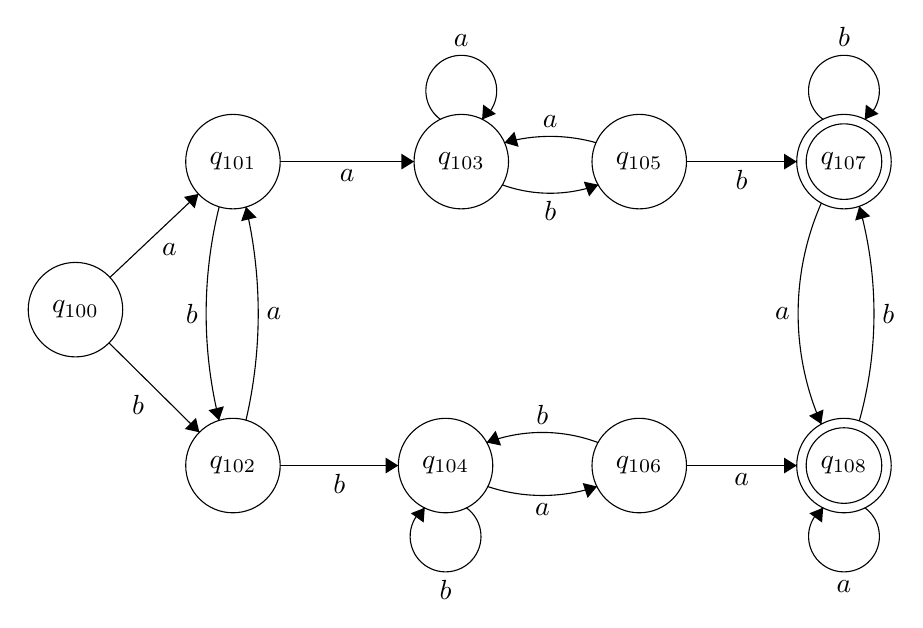
\begin{tikzpicture}[scale=0.2]
        \tikzstyle{every node}+=[inner sep=0pt]
        \draw [black] (3.2,-18.5) circle (3);
        \draw (3.2,-18.5) node {$q_{100}$};
        \draw [black] (13.2,-9.1) circle (3);
        \draw (13.2,-9.1) node {$q_{101}$};
        \draw [black] (13.2,-28.4) circle (3);
        \draw (13.2,-28.4) node {$q_{102}$};
        \draw [black] (27.7,-9.1) circle (3);
        \draw (27.7,-9.1) node {$q_{103}$};
        \draw [black] (26.7,-28.4) circle (3);
        \draw (26.7,-28.4) node {$q_{104}$};
        \draw [black] (39,-9.1) circle (3);
        \draw (39,-9.1) node {$q_{105}$};
        \draw [black] (39,-28.4) circle (3);
        \draw (39,-28.4) node {$q_{106}$};
        \draw [black] (52,-9.1) circle (3);
        \draw (52,-9.1) node {$q_{107}$};
        \draw [black] (52,-9.1) circle (2.4);
        \draw [black] (52,-28.4) circle (3);
        \draw (52,-28.4) node {$q_{108}$};
        \draw [black] (52,-28.4) circle (2.4);
        \draw [black] (5.39,-16.45) -- (11.01,-11.15);
        \fill [black] (11.01,-11.15) -- (10.09,-11.34) -- (10.77,-12.07);
        \draw (9.16,-14.28) node [below] {$a$};
        \draw [black] (5.33,-20.61) -- (11.07,-26.29);
        \fill [black] (11.07,-26.29) -- (10.85,-25.37) -- (10.15,-26.08);
        \draw (7.18,-23.93) node [below] {$b$};
        \draw [black] (16.2,-28.4) -- (23.7,-28.4);
        \fill [black] (23.7,-28.4) -- (22.9,-27.9) -- (22.9,-28.9);
        \draw (19.95,-28.9) node [below] {$b$};
        \draw [black] (14.027,-11.983) arc (13.12114:-13.12114:29.811);
        \fill [black] (14.03,-11.98) -- (13.72,-12.88) -- (14.7,-12.65);
        \draw (15.31,-18.75) node [right] {$a$};
        \draw [black] (12.325,-25.532) arc (-166.07551:-193.92449:28.183);
        \fill [black] (12.32,-25.53) -- (12.62,-24.64) -- (11.65,-24.88);
        \draw (11,-18.75) node [left] {$b$};
        \draw [black] (16.2,-9.1) -- (24.7,-9.1);
        \fill [black] (24.7,-9.1) -- (23.9,-8.6) -- (23.9,-9.6);
        \draw (20.45,-9.6) node [below] {$a$};
        \draw [black] (26.377,-6.42) arc (234:-54:2.25);
        \draw (27.7,-1.85) node [above] {$a$};
        \fill [black] (29.02,-6.42) -- (29.9,-6.07) -- (29.09,-5.48);
        \draw [black] (28.023,-31.08) arc (54:-234:2.25);
        \draw (26.7,-35.65) node [below] {$b$};
        \fill [black] (25.38,-31.08) -- (24.5,-31.43) -- (25.31,-32.02);
        \draw [black] (36.323,-29.732) arc (-71.42721:-108.57279:10.903);
        \fill [black] (36.32,-29.73) -- (35.41,-29.51) -- (35.72,-30.46);
        \draw (32.85,-30.8) node [below] {$a$};
        \draw [black] (36.402,-10.572) arc (-70.06975:-109.93025:8.953);
        \fill [black] (36.4,-10.57) -- (35.48,-10.37) -- (35.82,-11.31);
        \draw (33.35,-11.61) node [below] {$b$};
        \draw [black] (30.438,-7.898) arc (105.71254:74.28746:10.753);
        \fill [black] (30.44,-7.9) -- (31.34,-8.16) -- (31.07,-7.2);
        \draw (33.35,-7) node [above] {$a$};
        \draw [black] (29.309,-26.942) arc (110.6441:69.3559:10.044);
        \fill [black] (29.31,-26.94) -- (30.23,-27.13) -- (29.88,-26.19);
        \draw (32.85,-25.8) node [above] {$b$};
        \draw [black] (42,-28.4) -- (49,-28.4);
        \fill [black] (49,-28.4) -- (48.2,-27.9) -- (48.2,-28.9);
        \draw (45.5,-28.9) node [below] {$a$};
        \draw [black] (53.323,-31.08) arc (54:-234:2.25);
        \draw (52,-35.65) node [below] {$a$};
        \fill [black] (50.68,-31.08) -- (49.8,-31.43) -- (50.61,-32.02);
        \draw [black] (50.677,-6.42) arc (234:-54:2.25);
        \draw (52,-1.85) node [above] {$b$};
        \fill [black] (53.32,-6.42) -- (54.2,-6.07) -- (53.39,-5.48);
        \draw [black] (50.563,-25.771) arc (-156.26833:-203.73167:17.445);
        \fill [black] (50.56,-25.77) -- (50.7,-24.84) -- (49.78,-25.24);
        \draw (48.59,-18.75) node [left] {$a$};
        \draw [black] (52.974,-11.936) arc (15.5733:-15.5733:25.382);
        \fill [black] (52.97,-11.94) -- (52.71,-12.84) -- (53.67,-12.57);
        \draw (54.41,-18.75) node [right] {$b$};
        \draw [black] (42,-9.1) -- (49,-9.1);
        \fill [black] (49,-9.1) -- (48.2,-8.6) -- (48.2,-9.6);
        \draw (45.5,-9.6) node [below] {$b$};
    \end{tikzpicture}
    \caption{$M'$}
\end{figure}

\newpage
Actually we can merge $q_{107}$ and $q_{108}$ if we want to acquire in order to minimize a little bit more. This will changed nothing:
\begin{figure}[h!]
    \centering
    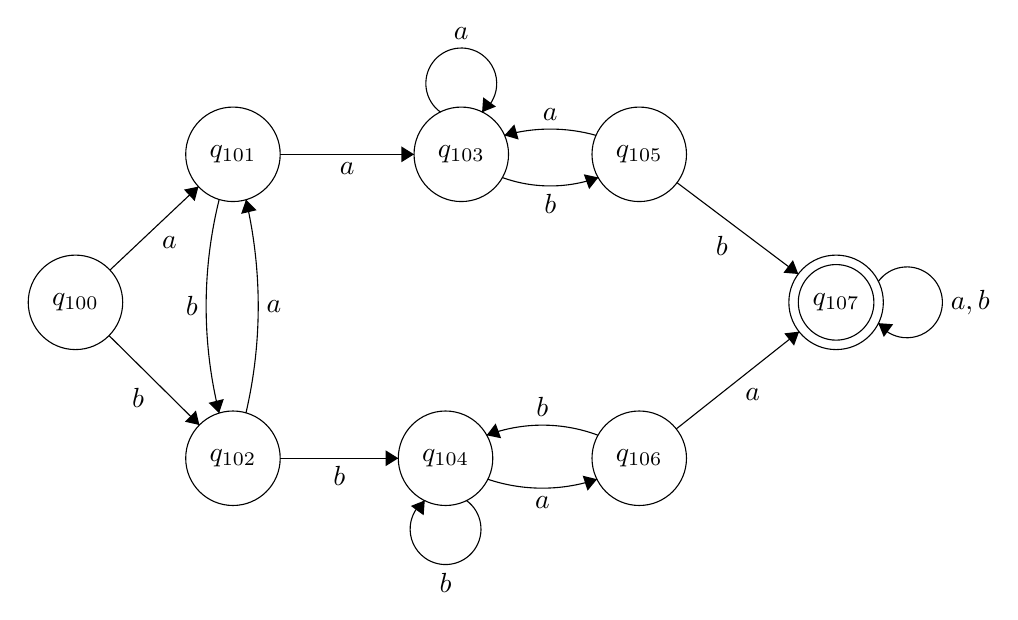
\begin{tikzpicture}[scale=0.2]
        \tikzstyle{every node}+=[inner sep=0pt]
        \draw [black] (3.2,-18) circle (3);
        \draw (3.2,-18) node {$q_{100}$};
        \draw [black] (13.2,-8.6) circle (3);
        \draw (13.2,-8.6) node {$q_{101}$};
        \draw [black] (13.2,-27.9) circle (3);
        \draw (13.2,-27.9) node {$q_{102}$};
        \draw [black] (27.7,-8.6) circle (3);
        \draw (27.7,-8.6) node {$q_{103}$};
        \draw [black] (26.7,-27.9) circle (3);
        \draw (26.7,-27.9) node {$q_{104}$};
        \draw [black] (39,-8.6) circle (3);
        \draw (39,-8.6) node {$q_{105}$};
        \draw [black] (39,-27.9) circle (3);
        \draw (39,-27.9) node {$q_{106}$};
        \draw [black] (51.5,-18) circle (3);
        \draw (51.5,-18) node {$q_{107}$};
        \draw [black] (51.5,-18) circle (2.4);
        \draw [black] (5.39,-15.95) -- (11.01,-10.65);
        \fill [black] (11.01,-10.65) -- (10.09,-10.84) -- (10.77,-11.57);
        \draw (9.16,-13.78) node [below] {$a$};
        \draw [black] (5.33,-20.11) -- (11.07,-25.79);
        \fill [black] (11.07,-25.79) -- (10.85,-24.87) -- (10.15,-25.58);
        \draw (7.18,-23.43) node [below] {$b$};
        \draw [black] (16.2,-27.9) -- (23.7,-27.9);
        \fill [black] (23.7,-27.9) -- (22.9,-27.4) -- (22.9,-28.4);
        \draw (19.95,-28.4) node [below] {$b$};
        \draw [black] (14.027,-11.483) arc (13.12114:-13.12114:29.811);
        \fill [black] (14.03,-11.48) -- (13.72,-12.38) -- (14.7,-12.15);
        \draw (15.31,-18.25) node [right] {$a$};
        \draw [black] (12.325,-25.032) arc (-166.07551:-193.92449:28.183);
        \fill [black] (12.32,-25.03) -- (12.62,-24.14) -- (11.65,-24.38);
        \draw (11,-18.25) node [left] {$b$};
        \draw [black] (16.2,-8.6) -- (24.7,-8.6);
        \fill [black] (24.7,-8.6) -- (23.9,-8.1) -- (23.9,-9.1);
        \draw (20.45,-9.1) node [below] {$a$};
        \draw [black] (26.377,-5.92) arc (234:-54:2.25);
        \draw (27.7,-1.35) node [above] {$a$};
        \fill [black] (29.02,-5.92) -- (29.9,-5.57) -- (29.09,-4.98);
        \draw [black] (28.023,-30.58) arc (54:-234:2.25);
        \draw (26.7,-35.15) node [below] {$b$};
        \fill [black] (25.38,-30.58) -- (24.5,-30.93) -- (25.31,-31.52);
        \draw [black] (36.323,-29.232) arc (-71.42721:-108.57279:10.903);
        \fill [black] (36.32,-29.23) -- (35.41,-29.01) -- (35.72,-29.96);
        \draw (32.85,-30.3) node [below] {$a$};
        \draw [black] (36.402,-10.072) arc (-70.06975:-109.93025:8.953);
        \fill [black] (36.4,-10.07) -- (35.48,-9.87) -- (35.82,-10.81);
        \draw (33.35,-11.11) node [below] {$b$};
        \draw [black] (30.438,-7.398) arc (105.71254:74.28746:10.753);
        \fill [black] (30.44,-7.4) -- (31.34,-7.66) -- (31.07,-6.7);
        \draw (33.35,-6.5) node [above] {$a$};
        \draw [black] (29.309,-26.442) arc (110.6441:69.3559:10.044);
        \fill [black] (29.31,-26.44) -- (30.23,-26.63) -- (29.88,-25.69);
        \draw (32.85,-25.3) node [above] {$b$};
        \draw [black] (41.35,-26.04) -- (49.15,-19.86);
        \fill [black] (49.15,-19.86) -- (48.21,-19.97) -- (48.83,-20.75);
        \draw (46.2,-23.45) node [below] {$a$};
        \draw [black] (41.4,-10.4) -- (49.1,-16.2);
        \fill [black] (49.1,-16.2) -- (48.76,-15.32) -- (48.16,-16.12);
        \draw (44.25,-13.8) node [below] {$b$};
        \draw [black] (54.18,-16.677) arc (144:-144:2.25);
        \draw (58.75,-18) node [right] {$a,b$};
        \fill [black] (54.18,-19.32) -- (54.53,-20.2) -- (55.12,-19.39);
    \end{tikzpicture}
    \caption{$M'_2$}
\end{figure}


\subsection*{d)}

\subsubsection*{Tracing in NFA}

\begin{align*}
    (q_0, bbabb) &\vdash_M (q_1, babb)\\
                 &\vdash_M (q_6, abb)\\
\end{align*}
This way is failed.
\begin{align*}
    (q_0, bbabb) &\vdash_M (q_1, bbabb)\\
                 &\vdash_M (q_6, babb)\\
                 &\vdash_M (q_7, abb)\\
                 &\vdash_M (q_8, abb)\\
                 &\vdash_M (q_9, bb)\\
\end{align*}
This way is failed.
\begin{align*}
    (q_0, bbabb) &\vdash_M (q_1, babb)\\
                 &\vdash_M (q_0, babb)\\
                 &\vdash_M (q_1, abb)\\
                 &\vdash_M (q_0, abb)\\
                 &\vdash_M (q_1, bb)\\
                 &\vdash_M (q_0, bb)\\
                 &\vdash_M (q_1, b)\\
                 &\vdash_M (q_0, b)\\
                 &\vdash_M (q_1, e)\\
\end{align*}
This way is failed.

Actually there is a no way to accept this string. In other words, $w'$ \textbf{cannot be accepted} by NFA $M$. It can be more clearly seen in DFA.

\subsubsection*{Tracing in DFA}

\begin{align*}
    (q_{100}, bbabb) &\vdash_M (q_{102}, babb)\\
                     &\vdash_M (q_{104}, abb)\\
                     &\vdash_M (q_{106}, bb)\\
                     &\vdash_M (q_{104}, b)\\
                     &\vdash_M (q_{104}, e)\\
\end{align*}

\noindent String $w'$ is \textbf{not accepted} by DFA $M'$ because the automata is not stopped at the one of the final states.




\newpage
\section*{Answer 2}

\subsection*{a)}

\quad If $L_1$ is a regular language, it should satisfy pumping lemma. According to pumping lemma, if $L_1$ is regular, there should be an integer $p \geq 1$ such that $w = a^mb^n \in L_1$ with $|w| \geq p$ can be written as $w = xyz$ such that:
\begin{itemize}
  \item $|y| > 0$,
  \item $|xy| < p$, and
  \item $xy^iz \in L_1$ for each $i \geq 0$.
\end{itemize}

\noindent When we focus on $y$, there are 4 possible $y$, while $k, l \geq 1$:
\begin{enumerate}
  \item $y = e$
  \item $y = a^k$
  \item $y = b^l$
  \item $y = a^kb^l$
\end{enumerate}

\noindent We can notice that there is not $y$ such that satisfies the conditions of pumping lemma. 
\begin{enumerate}
  \item $y \neq e$, from pumping lemma itself. (Contradiction)
  \item $y \neq a^k$, $y$ cannot include \textit{some} $a$: There are some situations that is valid but not all situation is valid. If the $m = n + 1$, $m \ngtr n$ when $i = 0$ for all $y = a^k$, while $k \geq 1$. (Contradiction)
  \item $y \neq b^l$, $y$ cannot include \textit{some} $b$: $m \ngtr n$ when for some $i > 0$. (Contradiction)
  \item $y \neq a^kb^l$, $y$ cannot include both \textit{some} $a$ and \textit{some} $b$: New strings out of pattern are generated (Example: $aaabbbaabb$). (Contradiction)
\end{enumerate}

\noindent Since all possible $y$ cause contradictions (at some points), which means that there is no integer $p$ that $L_1$ is \textbf{not regular language} according to pumping lemma. According to \textit{Theorem 2.3.1} in the textbook, languages accepted by finite automata are closed under complementation. So, $\overline{L_1}$ is also \textbf{not regular} language which is $L_2$

So, $L_2$ is \textbf{not regular} language.

\subsection*{b)}

\subsubsection*{$L_4$ is not regular}

\quad $L_4$ defines a language whose strings include equal number of $a$'s and $b$'s where $a$'s are located before $b$'s. We can use pumping lemma to show that $L_4$ is not regular.

Assume $L_4$ is regular languages. Then there should be an integer $p \geq 1$ such that $w = a^nb^n \in L_4$ with $|w| \geq p$ can be written as $w = xyz$ such that:
\begin{itemize}
  \item $|y| > 0$,
  \item $|xy| < p$, and
  \item $xy^iz \in L_4$ for each $i \geq 0$.
\end{itemize}

If $y = a^i$ for some $i > 0$, $xz = a^{n-i}b^n \notin L_4$ for $y^0 = e$, contradicting theorem. In other words, there is not any $y$ that satisfies $xy^iz \in L_4$ for each $i \geq 0$. New strings, $xy^iz$, either are out of pattern or does not have same number of $a$'s and $b$'s.

So, $L_4$ is \textbf{not regular} language according to pumping lemma.

\subsubsection*{$L_5$ is regular}

\quad In $L_5$, it stated that $m, n \in \mathbb{N}$, which means $m, n \geq 0$. So, $L_5$ can be expressed as:
\begin{equation*}
  L_5 = a^*b^*
\end{equation*}
because of the definition of \href{https://en.wikipedia.org/wiki/Kleene_star}{Kleene star} (Kleene star basically means \textit{zero or more occurences}).

So, it means that $L_5$ has a regular expression. If there is certain regular expression for a language, that language is regular language (It is also stated book in page 50: \textit{Regular languages are all languages that can be described by regular expressions.}).

Therefore, $L_5$ is \textbf{regular}.

\subsubsection*{$L_6$ is regular}

\quad Again, since $L_6$ is represented by certain regular expression, $L_6$ is regular.

\subsubsection*{$L_4 \cup L_5 \cup L_6$ is regular}

\quad At that point, we know that:
\begin{itemize}
  \item $L_4$ is not regular
  \item $L_5$ is regular
  \item $L_6$ is regular
\end{itemize}

If all of them was regular, we can say that the union of them is also regular because the languages are closed under union. However, $L_4$ is not regular.

When we focus on $L_4 \cup L_5$, we can notice that $L_4$ is subset of $L_5$, $L_4 \subset L_5$. So their union should be $L_5$:
\begin{equation*}
  L_4 \cup L_5 = L_5
\end{equation*}
So
\begin{equation*}
  L_4 \cup L_5 \cup L_6 = L_5 \cup L_6
\end{equation*}

So, according to \textit{Theorem 2.3.1} in the textbook, languages accepted by finite automata are closed under union. So, $L_5 \cup L_6$ is also \textbf{regular}.

Finally, we can say that $L_4 \cup L_5 \cup L_6$ is \textbf{regular}.

\end{document}
